\documentclass[11pt,a4paper]{article}

% Define page geometry
\usepackage{geometry} \geometry{left=2.2cm, right=2.2cm, top=2.2cm, bottom=2cm}
\parskip 0.15cm 
\setlength{\parindent}{0cm} 
\usepackage{pdflscape}
\usepackage[document]{ragged2e}

% Text formatting
\usepackage[T1]{fontenc}  % Set font

\usepackage{lineno}  % Line numbers

\usepackage{amssymb}  % Symbols
\usepackage{textcomp}
\newcommand{\textapprox}{\raisebox{0.5ex}{\texttildelow}}  % Command for a good tilde

\linespread{1.25}  % Linespacing

\usepackage{xcolor} \newcommand{\todo}[1]{\textcolor{red}{\textbf{#1}}}   %

% Tables
\usepackage{multirow} \setlength{\tabcolsep}{4pt}

% Image handling
\usepackage{graphicx} 

\makeatletter \g@addto@macro\@floatboxreset\centering  
\makeatother

\graphicspath{ {img/} }  % Define image path

\usepackage{subfig}  % Compound figures

\usepackage{float}  % Precise figure location

% Bibliography management
\usepackage[style=authoryear, natbib=true, backend=biber]{biblatex}
\addbibresource{lidar.bib}

% Links within document, nice figure formatting
\usepackage[breaklinks]{hyperref} \definecolor{links}{RGB}{0,0,0} \hypersetup{
	breaklinks, colorlinks=true, linkcolor=links, anchorcolor=links,
	citecolor=links, filecolor=links, menucolor=links, runcolor=links,
	urlcolor=links, pdfauthor={John L. Godlee} }
	\def\subsectionautorefname{section} \def\subsubsectionautorefname{section}

\newcommand{\beginsupplement}{% 
	\setcounter{table}{0}
	\renewcommand{\thetable}{S\arabic{table}}% 
	\setcounter{figure}{0}
	\renewcommand{\thefigure}{S\arabic{figure}}% 
}
     
% Variables

\newcommand{\titletext}{Terrestrial laser scanning}

\begin{document}

{\Large{Title: \titletext{}}}


\section*{Abstract}

\section{Introduction}

The characterization of tree canopy structure in wooded ecosystems constitutes a long-standing field of research that has been fundamental to interpreting, modelling, and improving understanding of ecosystem function \citep{Watt1947, Whittaker1969, Horn1971, Maarel1996}. Variation in canopy structure describes the spatial distribution and density of canopy foliage, which itself comprises the primary interface between trees, the atmosphere and sunlight. It is therefore essential to understand the drivers of variation in canopy structure to improve modelling efforts of earth-atmosphere carbon fluxes and community assembly \citep{}. 

At continental scales, variation in canopy height and canopy cover, two coarse measures of canopy structure both of which have been shown to affect woody productivity and correlate with woody biomass \citep{}, can largely be explained by climate and edaphic data \citep{SOME-GEDI}. At the scale of a single tree community however, where variation in climate and soil may be negligible, variation in canopy structure is thought to be affected principally by the tree canopy species assemblage \citep{}, and community history \citep{}. However, empirical testing of these mechanisms thought to drive canopy structure in natural wooded ecosystems remains sparse across many biomes \citep{}.

Following established biodiversity-ecosystem function theory, the niche partitioning of canopy space, i.e. the spatial complementarity of individual tree canopies, hereafter referred to as `crown complementarity', is thought to be a key mechanism underlying positive biodiversity-productivity effects in wooded ecosystems \citep{Pretzsch2014, Barry2019}. Biodiversity-ecosystem function theory predicts that canopy space occupation and thus canopy complexity and foliage density should increase with tree diversity, thus increasing standing biomass and woody productivity, as coexisting species must occupy non-identical niche space to avoid competitive exclusion \citep{}. 

While much work in the field of forest management has been done to test biotic drivers of tree canopy structure in temperate and boreal forests \citep{}, similar work in the tropics is comparatively scarce \citep{}. In dry tropical woodlands especially, tree canopy structure and its effect on ecosystem function has received little attention, possibly due to the misplaced assumption that woody productivity in these ecosystems does not represent a globally significant carbon flux \citep{}, or that tree canopies in these smaller stature woodlands do not interact and compete for resources to the same degree as in large stature forests \citep{}. In recent years however, it has been shown that dry tropical woodlands represent the largest uncertainty in our estimates of the terrestrial carbon cycle \citep{Quere2018, Ahlstrom2015}. \citet{Sitch2015} demonstrated the dominant role of the dry tropics in driving variability in the terrestrial carbon sink, and showed that the dry tropics are the fastest increasing component of the terrestrial carbon sink. Part of this uncertainty arises from our lacking a nuanced understanding of how species composition and structure affect ecosystem function in these ecosystems, which underpins the Dynamic Global Vegetation Models (DGVMs) fed into global carbon dynamics models. This knowledge gap prompts further research of the biotic drivers of variation in productivity in the dry tropics, of which variation in canopy structure is a constituent part \citep{}.

In addition to driving variation in woody productivity and biomass, canopy structure is also expected to affect understorey biomass. A more open tree canopy which provides more light to the ground can encourage understorey growth. In mesic savannas an open tree canopy is maintained via a positive feedback where increased grassy biomass as a result of a more open canopy increases the frequency and intensity of fires which serve to maintain the open canopy \citep{}. To elucidate the tipping points which determine when open savanna becomes forest, it is necessary therefore to understand how canopy structure affects grassy biomass. This line of enquiry is pertinent as multiple studies have reported increases in woody biomass across tropical savannas \citep{}. 

Canopy structure is multi-dimensional and has previously been explained using a plethora of metrics that originated in forest and community ecology \citep{}. Assessments of canopy structure in the dry tropical have most often modelled tree canopies as a series of ellipses (2D) or ellipsoids (3D) \citep{}. Measurements of this kind are time consuming and present a gross over-simplification of canopy structure \citep{}. Alternatively, canopy cover is often measured using indirect optical methods which partition sky from canopy material, i.e. with hemispherical photography or the commonly used LAI-2000, providing a 2D representation of the canopy that is a simplification in other ways. In recent years, particularly in temperate and boreal forests, LiDAR (Light Detection And Ranging) has emerged as a suitable technology for rapidly and precisely assessing canopy structure in 3D, conserving the complexity of the canopy that is required to understand it's multi-dimensional structure \citep{}.

In this study we applied terrestrial LiDAR techniques to mesic savannas at two sites in southern Africa, with the aim of increasing our understanding of how tree canopy structure is affected by tree neighbourhood diversity and stand structure. We also investigated how this variation in canopy structure affects understorey grassy biomass. Our overarching contention is that assemblages of greater tree diversity and greater stand structural diversity allow greater canopy complexity and foliage density, resulting in higher productivity, greater woody biomass, and a lower understorey biomass as a result of canopy light exclusion. 

\section{Materials and methods}

\subsection{Study sites}

Measurements were conducted at two sites, the first in Bicuar National Park, southwest Angola (S15.1$^\circ$, E14.8$^\circ$), and the second in Kilwa District, southeast Tanzania (S9.0$^\circ$, E39.0$^\circ$) (\autoref{map}).

\begin{figure}[H]
\centering
	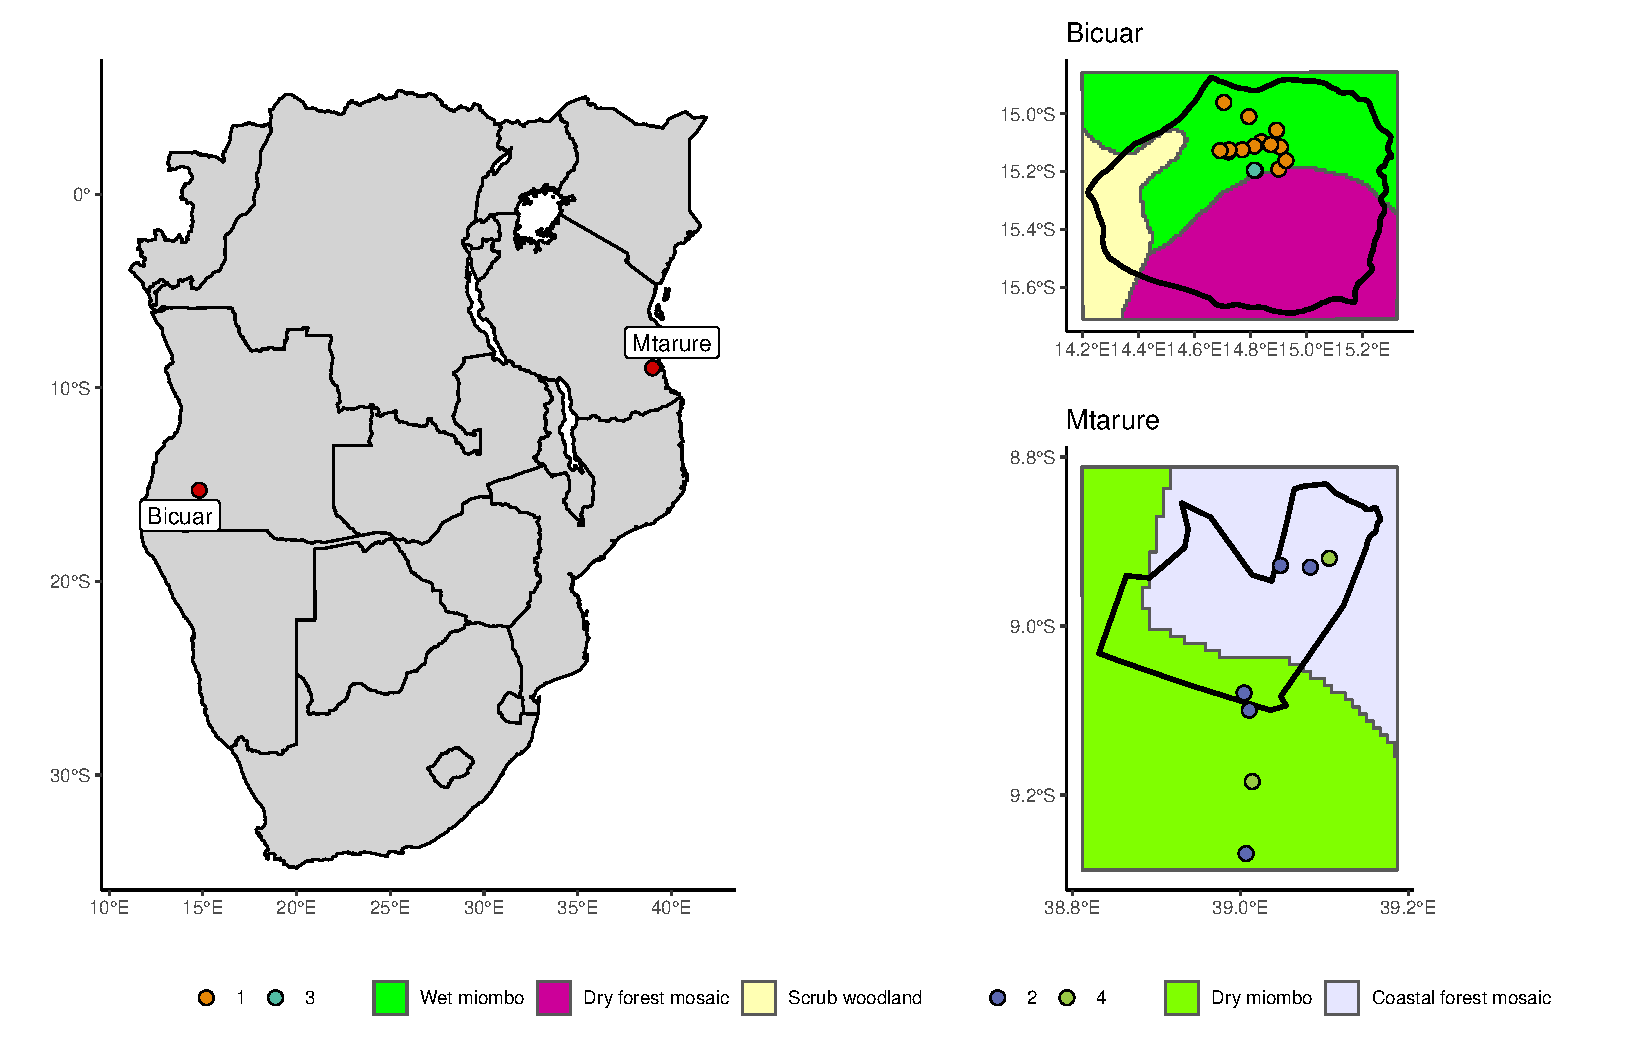
\includegraphics[width=\textwidth]{map}
	\caption{Location of study sites within southern Africa (a), and of 1 ha plots within each site. The blue polygons denote the boundaries of protected areas which encompass the majority of study sites, Bicuar National Park in Angola (b), and Mtarure Forest Reserve in Tanzania (c).}
	\label{map}
\end{figure}

\subsection{Field measurements}

Fieldwork was conducted between February and April at both sites, during the peak growth period of each site, in order to capture the highest leafy volume in the canopy and the largest grassy volume in the understorey.

At each site, a number of 1 ha permanent plots were sampled. In Angola, 15 plots were sampled, while in Tanzania, seven were sampled, following the curtailment of fieldwork due to COVID-19 travel restrictions. Each permanent plot was further subdivided into nine 10 m diameter circular subplots arranged in a regular grid, with a buffer from the plot edge (\autoref{subplot}).

\begin{figure}[H]
\centering
	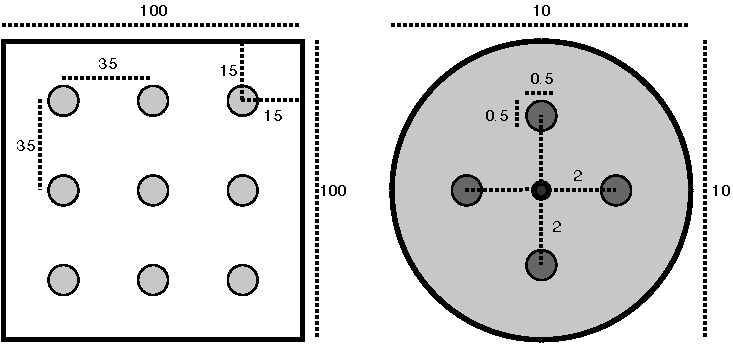
\includegraphics[width=\textwidth]{subplot}
	\caption{The layout of 10 m diameter subplots within each 1 ha square plot. Each subplot is situated inside a 15 m buffer from the plot edge, with 35 m between subplot centres. Subplots are arranged in a 3x3 grid. Disc-pasture measurements and biomass samples are located in cardinal directions 2 m from the centre of the subplot. All distances are in metres.}
	\label{subplot}
\end{figure}

For each subplot, we measured all woody stems >5 cm trunk diameter with canopy material inside the subplot. We identified each stem to species and measured trunk diameter (diameter at breast height - 1.3 m), height to top of canopy material, canopy area calculated as an ellipse of two perpendicular crown diameter measurements, distance and direction of stem from the subplot centre.

At the centre of each subplot a photograph was taken with a Nikon D750 full-frame DSLR camera, with a Sigma 8 mm f/3.5 EX DG circular fisheye lens. This lens has an equisolid (equal area) projection, which avoids image distortion. The photo was taken facing directly to zenith, with the top of the camera facing to magnetic north, at a height of 1.3 m or above understorey vegetation, whichever was higher. Photos were captured under uniform light conditions as much as possible, either under overcast skies or early in the day before direct sunlight could be seen on the photo. 

\subsection{Terrestrial laser scanning}

Within each subplot, a variable number of scans were recorded using a Leica HDS6100 phase-shift terrestrial laser scanner (TLS). The number and position of scans within a subplot was determined by the arrangement and density of canopy material in the subplot. Scan positions were arranged to minimise shadows within the canopy, and to maximise canopy penetration. Number of scans per subplot ranged between one and five in both Angola and Tanzania. Registration of multiple scans from different locations around each subplot allows us to minimise the occlusion effect and improve canopy penetration.

\subsection{Data analysis}

\subsubsection{Scan processing}

Point clouds from scans in each subplot were registered and unified using Leica Cyclone (version 9.1). Targets from each scan were aligned using Cyclone's automatic target acquisition. 

Point clouds were voxelised to different voxel sizes depending on the application of the data. For grassy volume estimation we used 2 cm\textsuperscript{3} cubic voxels, while for subplot height profile estimation and gap fraction we used 5 cm\textsuperscript{3} voxels, and for whole plot canopy rugosity we used 10 cm\textsuperscript{3} voxels. Variation in voxel size reflects the variation in spatial scale of each analysis, and is bounded by the beam divergence of the scanner. Choosing voxels that are too small can result in pock-marked representations of surfaces that are especially problematic when estimating canopy structure at a larger scale, such as when estimating canopy top roughness, while voxels that are too large can result in an over-estimation of plant volume when estimating canopy foliage density, for example \citep{Cifuentes2014}. Voxels were classed as filled if they intersected with one or more points.

Partial object interceptions caused by phase-shift laser scanners can produce erroneous results and must be corrected for to accurately estimate canopy height, for example \citep{}. We used a noise reduction algorithm to discard points that appeared far from other points, which removed ghost points produced by partial interceptions and also removed many erroneous returns caused by airborne particles, which was common in our study site.

Ground points were classified using the Progressive Morphological Filter (PMF) from \citep{Zhang2003}. Point cloud height was then reclassified height based on this revised ground layer by measuring the vertical distance between the nearest ground point and each point.

Resultant points clouds had ~points, ~points after filtering, ~voxels after voxelisation.

We used ray-tracing (POV-ray) to calculate gap fraction from TLS scans at the centre of each subplot. Voxels were converted to cubes filling the voxel volume, with a ``camera'' placed at the subplot centre at 1.8 m height, at a height of 1.8 m. Used a fisheye lens with a view angle of 180 degrees, with matt black Cubes against a white background and no light source. The images produced by POV-ray were analysed using Hemiphot in an identical manner to the hemispherical photographs.

\subsection{Data analysis}


\section{Results}

\subsection{Vertical canopy complexity}

\subsection{Grassy biomass}

\subsection{Canopy rugosity}


\section{Discussion}



\section{Conclusion}

\printbibliography

%\section{Supplementary Material} \beginsupplement

\end{document}
